\chapter{Implementation}
\label{ch:impl}

We first built the pipeline as one Kaggle notebook of about fifty cells, arranged in eleven sections that follow the stages of Chapter~\ref{ch:method}. Two runs of that notebook are part of this submission: \texttt{mini-6\_working} (configuration A) and \texttt{mini-7-fixed} (configuration B). They use the same code with a different data mix and different settings. Later we moved the code into a Python package with a command-line runner and a web application, described in Section~\ref{sec:system}. In this chapter we go through the code one module at a time, showing the important parts (shortened, with print statements removed), write the main procedures as algorithms, list the settings of every configuration, and record the problems we ran into and how we solved them.

\section{Module Overview}
\label{sec:modules}

\begin{table}[!htbp]
\centering
\caption[Implementation modules]{Implementation modules and the notebook sections that realise them.}
\label{tab:modules}
\small
\begin{tabularx}{\textwidth}{@{}L{0.7cm}L{4.1cm}Y@{}}
\toprule
\textbf{\#} & \textbf{Module} & \textbf{Responsibility}\\
\midrule
M1 & Environment \& persistence & Install/pin libraries, set environment flags, resolve paths, find previously saved adapters\\
M2 & HH-RLHF loader \& parser & Download helpful-base, split dialogues into prompt / chosen / rejected\\
M3 & LMSYS loader \& parser & Read \texttt{train.csv}, validate columns, drop ties, decode JSON turns, map winners\\
M4 & Filtering, balancing \& splitting & Truncate-and-filter, per-source sampling, stratified split, text cleaning, dataset plots\\
M5 & Reward model & Build DeBERTa-v3 + LoRA, train with \texttt{RewardTrainer}, save/load\\
M6 & RM scoring \& evaluation & Single/batched scoring with NaN guards; per-source accuracy, gap and plots\\
M7 & DPO alignment & Load 4-bit TinyLlama, format chat prompts, train with \texttt{DPOTrainer}, save/load, curves\\
M8 & Generation \& comparison & Sample responses from base and DPO models, score both, report winner\\
M9 & Batch evaluation & 25 + 25 held-out prompts, per-source win rate and $\Delta$, headline figure, CSV export\\
M10 & Interactive demo & Read user prompts in a loop, compare live, log the session\\
\bottomrule
\end{tabularx}
\end{table}

\section{M1: Environment Setup and Persistence}
\label{sec:m1}

The libraries already installed on Kaggle were older than PEFT 0.19 required, \texttt{torchao} in particular. Our first cells therefore reinstall \texttt{torchao}~$\ge$~0.16, upgrade \texttt{transformers}, \texttt{trl}, \texttt{peft}, \texttt{bitsandbytes} and \texttt{accelerate}, and remove the old copies from \texttt{sys.modules}. We also switch off Weights \& Biases logging through environment variables before importing TRL, because a protobuf version clash in the Kaggle image made that import fail.

Kaggle empties \texttt{/kaggle/working} at the end of every session. To avoid retraining each time, a small helper (Listing~\ref{lst:persist}) looks for a saved adapter in the working folder and in any attached input dataset, and the training stage is skipped when one is found.

\begin{lstlisting}[caption={Locating previously saved adapters across Kaggle sessions.}, label={lst:persist}]
import os, glob
os.environ["WANDB_DISABLED"] = "true"
os.environ["WANDB_MODE"] = "disabled"

BASE_DIR = "/kaggle/working" if os.path.exists("/kaggle/working") else "./outputs"

def find_saved_model(model_dir_name):
    """Check the working dir first, then any attached Kaggle input dataset."""
    working_path = f"{BASE_DIR}/{model_dir_name}"
    if os.path.exists(f"{working_path}/adapter_config.json"):
        return working_path
    candidates = glob.glob(f"/kaggle/input/**/{model_dir_name}/adapter_config.json",
                           recursive=True)
    if candidates:
        return os.path.dirname(candidates[0])
    return working_path        # default path; its absence triggers training

REWARD_MODEL_PATH  = find_saved_model("reward_model")
FINETUNED_LLM_PATH = find_saved_model("finetuned_llm")
\end{lstlisting}

All random generators (\texttt{random}, NumPy, PyTorch CPU and CUDA) are seeded with \texttt{SEED = 42} for reproducible sampling and splitting.

\section{M2: HH-RLHF Loader and Parser}
\label{sec:m2}

An HH-RLHF row holds the whole conversation twice, once ending in the chosen reply and once in the rejected one. We take the prompt to be everything before the \emph{last} \verb|\n\nAssistant:| marker in the chosen copy, and each response to be what comes after that marker in its own copy (Listing~\ref{lst:hh}). Searching from the end (\texttt{rfind}) keeps the earlier turns of a multi-turn chat inside the prompt. A row without the marker is returned empty and dropped later; this removed 52 of the 43,835 rows.

\begin{lstlisting}[caption={Parsing HH-RLHF dialogues into the common schema.}, label={lst:hh}]
from datasets import load_dataset
hh_train = load_dataset("Anthropic/hh-rlhf", data_dir="helpful-base", split="train")

def parse_hh(example):
    chosen, rejected = example["chosen"], example["rejected"]
    tok = "\n\nAssistant:"
    if tok not in chosen or tok not in rejected:
        return {"prompt": "", "chosen": "", "rejected": "", "source": "hh_rlhf"}
    c_idx, r_idx = chosen.rfind(tok), rejected.rfind(tok)
    prompt        = chosen[:c_idx].strip()
    chosen_resp   = chosen[c_idx + len(tok):].strip()
    rejected_resp = rejected[r_idx + len(tok):].strip()
    if prompt.startswith("\n\nHuman:"):
        prompt = prompt[len("\n\nHuman:"):].strip()
    return {"prompt": prompt, "chosen": chosen_resp,
            "rejected": rejected_resp, "source": "hh_rlhf"}

parsed = hh_train.map(parse_hh, remove_columns=hh_train.column_names)
hh_records = [r for r in parsed if r["prompt"] and r["chosen"] and r["rejected"]]
# -> 43,783 valid records
\end{lstlisting}

\section{M3: LMSYS Loader and Parser}
\label{sec:m3}

In the LMSYS file the conversation fields are Python or JSON lists stored as text, and \texttt{pandas} sometimes turns empty cells into \texttt{NaN}. Our \texttt{safe\_parse} function tries \texttt{ast.literal\_eval} first, then \texttt{json.loads}, and as a last resort wraps the raw value in a list. We strip spaces from the column names and check that all expected columns exist before looping over rows. When a chat has several turns we keep only the last user message and the last two replies. The reason is that the earlier replies on side A and side B were written by \emph{different} models, so copying one side's history into the shared prompt would give the other side a context it never saw.

\begin{lstlisting}[caption={Parsing LMSYS Chatbot Arena rows into the common schema.}, label={lst:lmsys}]
import ast, json, pandas as pd

def safe_parse(x):
    if isinstance(x, list):
        return x
    try:
        return ast.literal_eval(x)
    except (ValueError, SyntaxError, TypeError):
        try:
            return json.loads(x)
        except Exception:
            return [str(x)]

def flatten_conversation(prompt_list, response_list):
    prompts, responses = safe_parse(prompt_list), safe_parse(response_list)
    if not prompts:
        return "", ""
    final_prompt   = str(prompts[-1]).strip()          # last user turn only
    final_response = str(responses[-1]).strip() if responses else ""
    return final_prompt, final_response

lmsys_df = pd.read_csv(DATA_PATH)
lmsys_df.columns = lmsys_df.columns.str.strip()
expected = {"winner_tie", "winner_model_a", "winner_model_b",
            "prompt", "response_a", "response_b"}
assert expected <= set(lmsys_df.columns)

lmsys_records, n_ties = [], 0
for row in lmsys_df.itertuples(index=False):
    if row.winner_tie == 1:
        n_ties += 1; continue
    prompt_a, resp_a = flatten_conversation(row.prompt, row.response_a)
    _,        resp_b = flatten_conversation(row.prompt, row.response_b)
    if   row.winner_model_a == 1: chosen, rejected = resp_a, resp_b
    elif row.winner_model_b == 1: chosen, rejected = resp_b, resp_a
    else: continue                                     # ambiguous row
    if chosen and rejected and prompt_a:
        lmsys_records.append({"prompt": prompt_a, "chosen": chosen,
                              "rejected": rejected, "source": "lmsys"})
# -> 39,678 valid records, 17,761 ties dropped
\end{lstlisting}

\section{M4: Filtering, Balancing and Stratified Splitting}
\label{sec:m4}

\subsection{Truncate-and-filter}
LMSYS replies are noticeably longer than HH-RLHF replies (Figure~\ref{fig:m6-dataset}). Our first version threw away any record with a field over 1,500 characters. Since multi-turn prompts are long, this quietly removed most multi-turn LMSYS chats, which was the very variety we wanted LMSYS for. The final version \emph{shortens} every field to 1,500 characters and only throws away records with a field under 20 characters.

\begin{lstlisting}[caption={Uniform truncate-and-filter applied to both sources.}, label={lst:filter}]
MAX_CHARS, MIN_CHARS = 1500, 20

def truncate_and_filter(r):
    p, c, x = r["prompt"], r["chosen"], r["rejected"]
    if not (p and c and x):
        return None
    p, c, x = p[:MAX_CHARS], c[:MAX_CHARS], x[:MAX_CHARS]
    if min(len(p), len(c), len(x)) < MIN_CHARS:
        return None
    return {**r, "prompt": p, "chosen": c, "rejected": x}

hh_clean    = [o for r in hh_records    for o in [truncate_and_filter(r)] if o]
lmsys_clean = [o for r in lmsys_records for o in [truncate_and_filter(r)] if o]
# -> HH-RLHF 40,502 ; LMSYS 36,452
\end{lstlisting}

\subsection{Balancing and stratified split}
After shuffling both cleaned lists with the fixed seed, we take a set number of records from each: 2,000 and 2,000 in configuration A, and 6,000 HH-RLHF with 2,000 LMSYS in configuration B. The heavier HH share in B tested our guess that the cleaner expert labels would give a stronger training signal. Algorithm~\ref{alg:split} shows how the split is made.

\begin{algobox}{Source-stratified train/validation/test split}\label{alg:split}
\begin{lstlisting}[style=algo]
Input: combined DataFrame $D$ with column source; target sizes $n_{tr}, n_{va}, n_{te}$
Output: disjoint splits $D_{tr}, D_{va}, D_{te}$, each containing every source
for each source $s$ in unique($D$.source) do
    $D_s \leftarrow$ rows of $D$ with source $= s$          // already shuffled
    $f \leftarrow |D_s| / |D|$                               // share of source s
    $t \leftarrow$ round($n_{tr} f$); $v \leftarrow$ round($n_{va} f$); $e \leftarrow$ round($n_{te} f$)
    append $D_s[0:t]$ to $D_{tr}$; $D_s[t:t+v]$ to $D_{va}$; $D_s[t+v:t+v+e]$ to $D_{te}$
end for
shuffle each of $D_{tr}, D_{va}, D_{te}$ with seed 42
if $|D_{va}| < 20$ or $|D_{te}| < 20$ then warn and fall back to a tail slice
return $D_{tr}, D_{va}, D_{te}$
\end{lstlisting}
\end{algobox}

Finally, all text fields are cleaned of unpaired UTF-16 surrogate characters, which occur in some LMSYS responses and crash the fast tokenisers:

\begin{lstlisting}[caption={Removing invalid surrogate characters before tokenisation.}, label={lst:clean}]
def clean_text(text):
    if not isinstance(text, str):
        return ""
    return text.encode("utf-8", errors="surrogatepass").decode("utf-8", errors="ignore")

for col in ["prompt", "chosen", "rejected"]:
    for df in (train_df, val_df, test_df):
        df[col] = df[col].apply(clean_text)
\end{lstlisting}

\subsection{Sample records}
Two training records from configuration B, one from each source, illustrate the normalised schema (truncated):

\begin{table}[!htbp]
\centering
\caption[Example training records]{Example normalised training records (abridged).}
\label{tab:samples}
\small
\begin{tabularx}{\textwidth}{@{}lX@{}}
\toprule
\multicolumn{2}{@{}l}{\textbf{Source: hh\_rlhf}}\\
Prompt & Human: Can you recommend me similar movies to The Mummy (1999), Jungle Cruise and Pirates of the Caribbean? Assistant: The Mummy and Jungle Cruise are both from Disney, so maybe Big Hero 6 or Moana? \ldots\\
Chosen & Ah! Then how about Ghostbusters, E.T.\ or Men in Black?\\
Rejected & I suppose Bambi and The Lion King come to mind.\\
\midrule
\multicolumn{2}{@{}l}{\textbf{Source: lmsys}}\\
Prompt & I'm trying to learn German\\
Chosen & That's great! Germans are known for their efficiency and precision, so learning their language can be a great asset. Here are some tips to help you get started: 1.\ Develop a consistent study plan and \ldots\\
Rejected & That's great! Learning a new language can be a rewarding and challenging experience. Here are some tips to help you get started with learning German: 1.\ Familiarize yourself with the German alphabet \ldots\\
\bottomrule
\end{tabularx}
\end{table}

The LMSYS example shows why crowd labels are noisy: the two responses are very similar in quality and the vote could plausibly have gone either way.

\section{M5: Reward Model}
\label{sec:m5}

\subsection{Model construction}
We load the reward model with \texttt{AutoModelForSequenceClassification} and \texttt{num\_labels=1}, in FP32 (Section~\ref{sec:impl-fixes} explains why). LoRA goes on DeBERTa's attention projections, which are called \texttt{query\_proj}, \texttt{key\_proj} and \texttt{value\_proj}, not the Llama names.

\begin{lstlisting}[caption={Building the DeBERTa-v3 reward model with LoRA (configuration A).}, label={lst:rmbuild}]
from transformers import AutoTokenizer, AutoModelForSequenceClassification
from peft import LoraConfig, get_peft_model, TaskType

RM_BASE_MODEL = "microsoft/deberta-v3-base"
rm_tokenizer = AutoTokenizer.from_pretrained(RM_BASE_MODEL)
rm_tokenizer.padding_side = "right"

rm_base = AutoModelForSequenceClassification.from_pretrained(
    RM_BASE_MODEL, num_labels=1,
    torch_dtype=torch.float32,          # FP16 gives NaN in disentangled attention
    device_map="auto")
rm_base.config.pad_token_id = rm_tokenizer.pad_token_id

rm_lora = LoraConfig(
    task_type=TaskType.SEQ_CLS,
    r=32, lora_alpha=64, lora_dropout=0.05,       # config B: r=64, alpha=128
    target_modules=["query_proj", "key_proj", "value_proj"],
    bias="none",
    modules_to_save=["pooler"])         # train AND save the pooler head
reward_model = get_peft_model(rm_base, rm_lora)
reward_model.enable_input_require_grads()   # needed with gradient checkpointing
reward_model.print_trainable_parameters()
# A: trainable params: 2,360,833 || all params: 186,783,746 || trainable%: 1.26
# B: trainable params: 4,130,305 || all params: 188,553,218 || trainable%: 2.19
\end{lstlisting}

\subsection{Training}
TRL's \texttt{RewardTrainer} does the tokenising itself: it builds (prompt, chosen) and (prompt, rejected) inputs, adds an end-of-sequence token, drops pairs over the length limit, and minimises the Bradley--Terry loss~\eqref{eq:rmloss}.

\begin{lstlisting}[caption={Reward-model training with TRL (configuration A).}, label={lst:rmtrain}]
from trl import RewardConfig, RewardTrainer
from datasets import Dataset

rm_train_ds = Dataset.from_pandas(train_df[["prompt", "chosen", "rejected"]])
rm_val_ds   = Dataset.from_pandas(val_df[["prompt", "chosen", "rejected"]])

rm_config = RewardConfig(
    output_dir=f"{BASE_DIR}/rm_checkpoints",
    num_train_epochs=2,                 # config B: 3
    per_device_train_batch_size=8, per_device_eval_batch_size=8,
    gradient_accumulation_steps=2, gradient_checkpointing=True,
    learning_rate=2e-5,                 # config B: 1e-5
    lr_scheduler_type="cosine", warmup_steps=100,   # config B: 200
    logging_steps=25, eval_strategy="steps", eval_steps=100,
    save_strategy="no", fp16=False, max_length=512,
    remove_unused_columns=False, report_to="none", optim="adamw_torch")

rm_trainer = RewardTrainer(model=reward_model, args=rm_config,
                           processing_class=rm_tokenizer,
                           train_dataset=rm_train_ds, eval_dataset=rm_val_ds)
rm_trainer.train()
reward_model.save_pretrained(REWARD_MODEL_PATH)
rm_tokenizer.save_pretrained(REWARD_MODEL_PATH)
json.dump(rm_trainer.state.log_history,
          open(f"{REWARD_MODEL_PATH}/training_log.json", "w"))
\end{lstlisting}

\section{M6: Reward Scoring and Per-Source Evaluation}
\label{sec:m6}

The scoring functions send inputs to whichever device actually holds the model (on a two-GPU machine \texttt{device\_map=\textquotedbl{}auto\textquotedbl{}} can put it on \texttt{cuda:1}). Every score is checked for NaN or infinity, and a warning is printed directly so that warning filters cannot hide it.

\begin{lstlisting}[caption={Batched reward scoring with device-safe placement and NaN guards.}, label={lst:score}]
@torch.no_grad()
def reward_batch(prompts, responses, max_len=512, batch_size=8):
    rm_device = next(reward_model.parameters()).device
    scores = []
    for i in range(0, len(prompts), batch_size):
        inputs = rm_tokenizer(prompts[i:i+batch_size], responses[i:i+batch_size],
                              truncation=True, max_length=max_len,
                              padding=True, return_tensors="pt").to(rm_device)
        raw = reward_model(**inputs).logits[:, 0].float()
        if (~torch.isfinite(raw)).any():
            print("WARNING: NaN/inf reward scores - check that DeBERTa is in FP32")
        scores.extend(raw.tolist())
    return scores
\end{lstlisting}

\begin{algobox}{Per-source reward-model evaluation}\label{alg:rmeval}
\begin{lstlisting}[style=algo]
Input: test split $D_{te}$, reward model $r_\phi$
Output: accuracy, mean chosen/rejected reward and gap for overall, HH and LMSYS subsets
for each subset $S \in \{D_{te},\ D_{te}[\text{source}=hh],\ D_{te}[\text{source}=lmsys]\}$ do
    $c \leftarrow$ reward_batch($S$.prompt, $S$.chosen);  $j \leftarrow$ reward_batch($S$.prompt, $S$.rejected)
    keep only indices where both $c_i$ and $j_i$ are finite
    acc $\leftarrow$ mean($c > j$);  gap $\leftarrow$ mean($c - j$)
    report $|S|$, mean($c$), mean($j$), gap, acc
end for
if mean chosen $>$ mean rejected (overall) then PASS
if $|$acc$_{hh}$ $-$ acc$_{lmsys}|$ $< 0.10$ then BALANCED else IMBALANCED
\end{lstlisting}
\end{algobox}

The evaluation also produces a $2\times3$ figure of chosen/rejected score histograms and reward-gap histograms for each subset (Chapter~\ref{ch:results}).

\section{M7: DPO Alignment}
\label{sec:m7}

\subsection{Loading the 4-bit policy}
The policy is loaded through an NF4 \texttt{BitsAndBytesConfig} with FP16 as the compute type, since the T4 has no BF16 arithmetic. Passing \texttt{torch\_dtype=float16} makes the layers that are not quantised (embeddings and output head) FP16 as well. \texttt{prepare\_model\_for\_kbit\_training} then moves the normalisation layers to FP32 and enables input gradients for checkpointing.

\begin{lstlisting}[caption={Loading TinyLlama-1.1B-Chat in 4-bit NF4.}, label={lst:policy}]
from transformers import AutoModelForCausalLM, BitsAndBytesConfig
from peft import prepare_model_for_kbit_training

POLICY_BASE_MODEL = "TinyLlama/TinyLlama-1.1B-Chat-v1.0"
policy_tokenizer = AutoTokenizer.from_pretrained(POLICY_BASE_MODEL)
if policy_tokenizer.pad_token is None:
    policy_tokenizer.pad_token = policy_tokenizer.eos_token

bnb_dpo = BitsAndBytesConfig(load_in_4bit=True, bnb_4bit_quant_type="nf4",
                             bnb_4bit_compute_dtype=torch.float16,
                             bnb_4bit_use_double_quant=True)
policy_model = AutoModelForCausalLM.from_pretrained(
    POLICY_BASE_MODEL, quantization_config=bnb_dpo,
    torch_dtype=torch.float16, device_map="auto")
policy_model = prepare_model_for_kbit_training(policy_model)
# Policy loaded. VRAM: 1.14 GB
\end{lstlisting}

\subsection{Preparing preference pairs}
Each prompt is wrapped in TinyLlama's chat template with the assistant prefix added, so DPO computes probabilities on the same format the model will see when answering. Configuration A draws 1,500 random training pairs (776 HH-RLHF, 724 LMSYS); configuration B draws 2,000 HH-RLHF and 1,000 LMSYS pairs. Both use 200 validation pairs.

\begin{lstlisting}[caption={Formatting DPO training pairs with the chat template.}, label={lst:dpofmt}]
def format_for_dpo(ex):
    prompt_text = policy_tokenizer.apply_chat_template(
        [{"role": "user", "content": ex["prompt"]}],
        tokenize=False, add_generation_prompt=True)
    return {"prompt": prompt_text, "chosen": ex["chosen"], "rejected": ex["rejected"]}

dpo_train_df = train_df.sample(n=min(1500, len(train_df)), random_state=SEED)
dpo_train_ds = Dataset.from_pandas(dpo_train_df[["prompt","chosen","rejected"]]) \
                      .map(format_for_dpo, remove_columns=["prompt","chosen","rejected"])
\end{lstlisting}

\subsection{DPO training}
We pass \texttt{DPOTrainer} the 4-bit model, a \texttt{peft\_config} and \texttt{ref\_model=None}. TRL then gets the reference probabilities by switching the LoRA adapters off for a moment, so a single copy of the base weights serves as both policy and reference.

\begin{lstlisting}[caption={DPO configuration and training (configuration A; configuration B values in comments).}, label={lst:dpotrain}]
from trl import DPOConfig, DPOTrainer

dpo_lora = LoraConfig(r=16, lora_alpha=32, lora_dropout=0.05,   # B: r=32, alpha=64
                      target_modules=["q_proj", "k_proj", "v_proj", "o_proj"],
                      # B adds: "gate_proj", "up_proj", "down_proj"
                      bias="none", task_type="CAUSAL_LM")

dpo_config = DPOConfig(
    output_dir=f"{BASE_DIR}/dpo_checkpoints",
    num_train_epochs=2,
    per_device_train_batch_size=4, per_device_eval_batch_size=4,
    gradient_accumulation_steps=4, gradient_checkpointing=True,
    learning_rate=5e-5,                 # B: 1e-5
    lr_scheduler_type="cosine", warmup_steps=19,   # B: 38
    logging_steps=20, eval_strategy="steps", eval_steps=150,
    save_strategy="no",                 # B: save every 150 steps,
                                        #    load_best_model_at_end=True
    bf16=False, fp16=False,
    beta=0.1,                           # B: 0.15
    max_length=512, remove_unused_columns=False, report_to="none",
    optim="paged_adamw_8bit")

dpo_trainer = DPOTrainer(model=policy_model, ref_model=None, args=dpo_config,
                         train_dataset=dpo_train_ds, eval_dataset=dpo_val_ds,
                         processing_class=policy_tokenizer, peft_config=dpo_lora)
dpo_trainer.train()
dpo_trainer.save_model(FINETUNED_LLM_PATH)
\end{lstlisting}

\section{M8: Generation and Side-by-Side Comparison}
\label{sec:m8}

For the evaluation we load a plain 4-bit base model and a second 4-bit copy carrying the saved DPO adapter, which together with the reward model use about 1.5\,GB of GPU memory. Both models sample with temperature 0.7, top-$p$ 0.9, repetition penalty 1.15 and at most 200 new tokens.

\begin{lstlisting}[caption={Generating and comparing base and DPO responses.}, label={lst:compare}]
@torch.no_grad()
def generate_response(model, prompt, max_new_tokens=200):
    chat_text = policy_tokenizer.apply_chat_template(
        [{"role": "user", "content": prompt}], tokenize=False, add_generation_prompt=True)
    device = next(model.parameters()).device
    inputs = policy_tokenizer(chat_text, return_tensors="pt", truncation=True,
                              max_length=512).to(device)
    out = model.generate(**inputs, max_new_tokens=max_new_tokens, do_sample=True,
                         temperature=0.7, top_p=0.9, repetition_penalty=1.15,
                         pad_token_id=policy_tokenizer.eos_token_id)
    return policy_tokenizer.decode(out[0, inputs["input_ids"].shape[1]:],
                                   skip_special_tokens=True).strip()

def compare_responses(user_prompt, verbose=True):
    base = generate_response(base_model, user_prompt)
    dpo  = generate_response(finetuned_model, user_prompt)
    s_base, s_dpo = reward_score(user_prompt, base), reward_score(user_prompt, dpo)
    return {"prompt": user_prompt, "base_response": base, "finetuned_response": dpo,
            "base_score": s_base, "finetuned_score": s_dpo, "delta": s_dpo - s_base}
\end{lstlisting}

\section{M9: Held-Out Batch Evaluation}
\label{sec:m9}

\begin{algobox}{Per-source DPO win-rate evaluation}\label{alg:dpoeval}
\begin{lstlisting}[style=algo]
Input: test split $D_{te}$, base policy $\pi_0$, aligned policy $\pi_{dpo}$, reward model $r_\phi$, $k = 25$
Output: win rate and mean $\Delta$ for overall, HH and LMSYS
$P_{hh} \leftarrow$ sample($k$ rows of $D_{te}$ with source $=$ hh, seed 42)
$P_{lm} \leftarrow$ sample($k$ rows of $D_{te}$ with source $=$ lmsys, seed 42)
for each prompt $x$ in $P_{hh} \cup P_{lm}$ do
    $y_0 \sim \pi_0(\cdot \mid x)$;  $y_1 \sim \pi_{dpo}(\cdot \mid x)$      // same sampling settings
    $\Delta_x \leftarrow r_\phi(x, y_1) - r_\phi(x, y_0)$
end for
for each group $G \in \{$all, hh, lmsys$\}$ do
    WR$_G \leftarrow$ mean($\Delta_x > 0$ for $x \in G$);   $\bar\Delta_G \leftarrow$ mean($\Delta_x$ for $x \in G$)
end for
save per-prompt results to batch_eval.csv; plot win rates, score histograms, sorted $\Delta$
\end{lstlisting}
\end{algobox}

\section{M10: Interactive Demonstration}
\label{sec:m10}

The last notebook cell is a live loop for demonstrations. A user types a prompt, both models answer, both answers are scored, and the cell prints the winner and the percentage change. Typing \texttt{quit}, \texttt{exit} or \texttt{q} stops the loop and saves the session to \texttt{interactive\_session.csv}. When the notebook is run with ``Run All'' there is no keyboard, so the cell catches the resulting \texttt{EOFError} and skips itself. The web application of Section~\ref{sec:system} replaces this loop with a proper interface.

\section{Hyper-parameters of the Two Configurations}
\label{sec:hparams}

\begin{table}[!htbp]
\centering
\caption[Reward-model hyper-parameters (A and B)]{Reward-model hyper-parameters for configurations A (mini-6) and B (mini-7).}
\label{tab:rm-hparams}
\small
\begin{tabularx}{\textwidth}{@{}L{5.2cm}ZZ@{}}
\toprule
\textbf{Hyper-parameter} & \textbf{Config.\ A} & \textbf{Config.\ B}\\
\midrule
Backbone & \multicolumn{2}{c}{microsoft/deberta-v3-base (FP32)}\\
Training pairs (HH / LMSYS) & 3,500 (1,750 / 1,750) & 7,000 (5,250 / 1,750)\\
LoRA rank $r$ / $\alpha$ / dropout & 32 / 64 / 0.05 & 64 / 128 / 0.05\\
LoRA targets & \multicolumn{2}{c}{query\_proj, key\_proj, value\_proj}\\
Extra trainable modules & \multicolumn{2}{c}{classifier (auto), pooler (\texttt{modules\_to\_save})}\\
Trainable parameters & 2.36M / 186.8M (1.26\%) & 4.13M / 188.6M (2.19\%)\\
Learning rate & $2\times10^{-5}$ & $1\times10^{-5}$\\
Epochs & 2 & 3\\
Per-device batch / grad.\ accumulation & 8 / 2 & 8 / 2\\
Effective batch (2 GPUs) & 32 & 32\\
Scheduler / warm-up steps & cosine / 100 & cosine / 200\\
Max sequence length & 512 & 512\\
Optimiser & AdamW (torch) & AdamW (torch)\\
Evaluation interval & 100 steps & 100 steps\\
\bottomrule
\end{tabularx}
\end{table}

\begin{table}[!htbp]
\centering
\caption[DPO hyper-parameters (A and B)]{DPO hyper-parameters for configurations A (mini-6) and B (mini-7).}
\label{tab:dpo-hparams}
\small
\begin{tabularx}{\textwidth}{@{}L{5.2cm}ZZ@{}}
\toprule
\textbf{Hyper-parameter} & \textbf{Config.\ A} & \textbf{Config.\ B}\\
\midrule
Policy & \multicolumn{2}{c}{TinyLlama/TinyLlama-1.1B-Chat-v1.0}\\
Quantisation & \multicolumn{2}{c}{4-bit NF4, double quant., FP16 compute}\\
Training pairs (HH / LMSYS) & 1,500 (776 / 724) & 3,000 (2,000 / 1,000)\\
LoRA rank $r$ / $\alpha$ / dropout & 16 / 32 / 0.05 & 32 / 64 / 0.05\\
LoRA targets & $q,k,v,o$ & $q,k,v,o$, gate, up, down\\
Trainable parameters (computed) & $\approx$4.5M (0.41\%) & $\approx$25.2M (2.3\%)\\
DPO $\beta$ & 0.10 & 0.15\\
Learning rate & $5\times10^{-5}$ & $1\times10^{-5}$\\
Per-device batch / grad.\ accumulation & 4 / 4 & 4 / 4\\
Optimisation steps (from training log) & $\approx$188 & $\approx$560\\
Scheduler / warm-up steps & cosine / 19 & cosine / 38\\
Checkpoint selection & final weights & best eval loss\\
Max sequence length & 512 & 512\\
Optimiser & \multicolumn{2}{c}{paged AdamW 8-bit, gradient checkpointing}\\
\bottomrule
\end{tabularx}
\end{table}

\section{From Notebook to a Working System}
\label{sec:system}

A notebook is convenient for experiments but awkward to reuse: cells depend on each other's variables, the code assumes Kaggle paths, and showing the result to someone means re-running half the notebook. Once the experiments were finished we reorganised the same code into a small system, \texttt{rlhf\_system}, with two entry points. The first is a command-line runner that executes the pipeline stage by stage. The second is a web application that loads the trained models and lets anyone compare the two chat models from a browser. The training logic is unchanged from the notebooks, so a model trained by either one can be loaded by the other.

\subsection{Package structure}

\begin{table}[!htbp]
\centering
\caption[Files of the packaged system]{Files of the packaged system and what each one does.}
\label{tab:package}
\small
\begin{tabularx}{\textwidth}{@{}L{3.6cm}Y@{}}
\toprule
\textbf{File} & \textbf{Role}\\
\midrule
\texttt{rlhf/config.py} & The settings of configurations A, B and \emph{local} as Python data classes, copied from the notebooks\\
\texttt{rlhf/data.py} & Stage 1: HH-RLHF and LMSYS loaders, \texttt{safe\_parse}, truncate-and-filter, per-source split; saves \texttt{train/val/test.csv}\\
\texttt{rlhf/models.py} & Loads and runs both models on CUDA, Apple MPS or CPU; reward scoring; base and DPO generation from one model copy\\
\texttt{rlhf/train.py} & Stage 2 (reward model) and Stage 3 (DPO); each is skipped if its adapter already exists\\
\texttt{rlhf/evaluate.py} & Stage 4: per-source reward-model accuracy, demo prompts, held-out win rates; writes \texttt{metrics.json}\\
\texttt{run\_pipeline.py} & Command line: \texttt{-{}-config A|B|local} and \texttt{-{}-stage data|rm|dpo|eval|all}\\
\texttt{app.py} & Web application (Gradio) with Compare, Results and About tabs\\
\texttt{models/} & Folder for adapters downloaded from Kaggle; these take priority over local runs\\
\bottomrule
\end{tabularx}
\end{table}

A complete run is a single command, for example \texttt{python run\_pipeline.py -{}-config A} on Kaggle, or \texttt{-{}-config local} on the laptop. Because each stage checks for its own output first, the same command also resumes a run that was interrupted.

\subsection{Running on three kinds of hardware}
The loader in \texttt{rlhf/models.py} checks what hardware is present and picks matching settings. On an NVIDIA GPU it uses exactly the notebook set-up: NF4 weights with FP16 compute. On an Apple Silicon Mac, where bitsandbytes is not available, TinyLlama is loaded in plain FP16 on the MPS backend. On a machine with neither it falls back to FP32 on the CPU, which is slow but works. The reward model always runs in FP32, for the reason given in Section~\ref{sec:impl-fixes}.

One detail matters a lot on an 8\,GB laptop. The base model and the DPO model differ only by the LoRA adapter, so the application keeps a single copy of TinyLlama and switches the adapter off when it needs the base model's answer (Listing~\ref{lst:policypair}). This halves the memory needed compared with loading two copies, as the notebook did.

\begin{lstlisting}[caption={One TinyLlama copy serves both the base and the DPO model.}, label={lst:policypair}]
class PolicyPair:
    def __init__(self, adapter_dir=None, device=None):
        self.device = device or pick_device()          # "cuda", "mps" or "cpu"
        model, self.tokenizer = load_policy_base(self.device)
        self.has_dpo = has_adapter(adapter_dir)
        if self.has_dpo:
            model = PeftModel.from_pretrained(model, str(adapter_dir))
        self.model = model.eval()

    def generate_base(self, prompt, **kw):
        if self.has_dpo:
            with self.model.disable_adapter():         # same weights, adapter off
                return self._generate(prompt, **kw)
        return self._generate(prompt, **kw)

    def generate_dpo(self, prompt, **kw):
        return self._generate(prompt, **kw)            # adapter on
\end{lstlisting}

\subsection{The local configuration}
The full configurations need a CUDA GPU. To have a version that trains on the team's own laptop, we added configuration \emph{local}: the method of configuration A on fewer pairs with shorter inputs (Table~\ref{tab:local-hparams}). On Kaggle the LMSYS file is attached as a competition dataset. Outside Kaggle the loader downloads the identical public copy from the HuggingFace Hub instead. The record counts it produced (43,783 valid HH-RLHF pairs, 39,678 valid LMSYS pairs, 17,761 ties removed) match the notebook exactly.

\begin{table}[!htbp]
\centering
\caption[Local configuration vs.\ configuration A]{Settings of the local configuration compared with configuration A.}
\label{tab:local-hparams}
\small
\begin{tabularx}{\textwidth}{@{}L{5.2cm}ZZ@{}}
\toprule
\textbf{Setting} & \textbf{Config.\ A (Kaggle T4)} & \textbf{Config.\ local (M1, 8 GB)}\\
\midrule
Pairs per source & 2,000 & 1,000\\
Train / val / test & 3,500 / 250 / 250 & 1,750 / 124 / 126\\
Reward-model epochs, LR & 2, $2\times10^{-5}$ & 1, $2\times10^{-5}$\\
Max input length (RM) & 512 tokens & 384 tokens\\
Policy precision & 4-bit NF4, FP16 compute & FP16 (no quantisation)\\
DPO pairs & 1,500 & 400\\
DPO batch $\times$ accumulation & 4 $\times$ 4 & 1 $\times$ 8\\
DPO max length & 512 tokens & 256 tokens\\
DPO epochs, LR, $\beta$ & 2, $5\times10^{-5}$, 0.1 & 1, $5\times10^{-5}$, 0.1\\
Held-out prompts per source & 25 & 15\\
Measured training time & $\approx$ 2.5--3 h (whole run) & RM 58 min, DPO 22 min, eval 12 min\\
\bottomrule
\end{tabularx}
\end{table}

\subsection{The web application}
Figure~\ref{fig:apparch} shows how a request travels through the application. When it starts, the application looks for trained adapters, first in \texttt{models/} (where downloaded Kaggle models go) and then in the pipeline's output folders, and loads TinyLlama once and the reward model once. Each click on \emph{Compare} produces two answers with the same sampling settings and seed, scores both, and shows the winner. If no adapters are found, the application still starts in a base-only mode and says so.

\begin{figure}[H]
\centering
\begin{tikzpicture}[
  box/.style={draw, thick, rounded corners=4pt, text width=3.2cm, minimum height=1.15cm, align=center, font=\footnotesize},
  arr/.style={-{Stealth[length=2.3mm]}, thick},
  lbl/.style={font=\scriptsize, fill=white, inner sep=1.5pt}]
\node[box, fill=boxA] (ui) at (0,0) {Browser\\(Compare tab)};
\node[box, fill=boxB] (srv) at (5.0,0) {\texttt{app.py}\\Gradio server};
\node[box, fill=boxC] (pol) at (10.2,1.6) {\texttt{PolicyPair}\\TinyLlama + DPO adapter};
\node[box, fill=boxD] (rm) at (10.2,-1.6) {\texttt{RewardModel}\\DeBERTa-v3 + adapter};
\node[box, fill=boxE] (disk) at (5.0,-3.2) {Adapters on disk\\\texttt{models/} or \texttt{outputs/}};
\draw[arr] ([yshift=6pt]ui.east) -- node[lbl, above=1pt]{prompt} ([yshift=6pt]srv.west);
\draw[arr] ([yshift=-6pt]srv.west) -- node[lbl, below=1pt]{verdict + answers} ([yshift=-6pt]ui.east);
\draw[arr] ([yshift=4pt]srv.east) |- node[lbl, pos=0.75, above]{base and DPO answers} (pol.west);
\draw[arr] ([yshift=-4pt]srv.east) |- node[lbl, pos=0.75, below]{two reward scores} (rm.west);
\draw[arr, dashed] (disk.north) -- node[lbl, right]{loaded at start-up} (srv.south);
\end{tikzpicture}
\caption[Web application request flow]{Flow of one comparison request through the web application.}
\label{fig:apparch}
\end{figure}

The interface has three tabs. \emph{Compare} (Figures~\ref{fig:ui-top} and~\ref{fig:ui-answers}) shows which models are loaded, a prompt box with example prompts, a coloured result banner, the two answers side by side with their reward scores, and a history of the session that can be saved as CSV. \emph{Results} (Figure~\ref{fig:ui-results}) reads \texttt{metrics.json} for the loaded models and shows the per-source tables of Chapter~\ref{ch:results}. \emph{About} (Figure~\ref{fig:ui-about}) summarises the pipeline and the Kaggle results for viewers who have not read this report.

\begin{figure}[H]
\centering
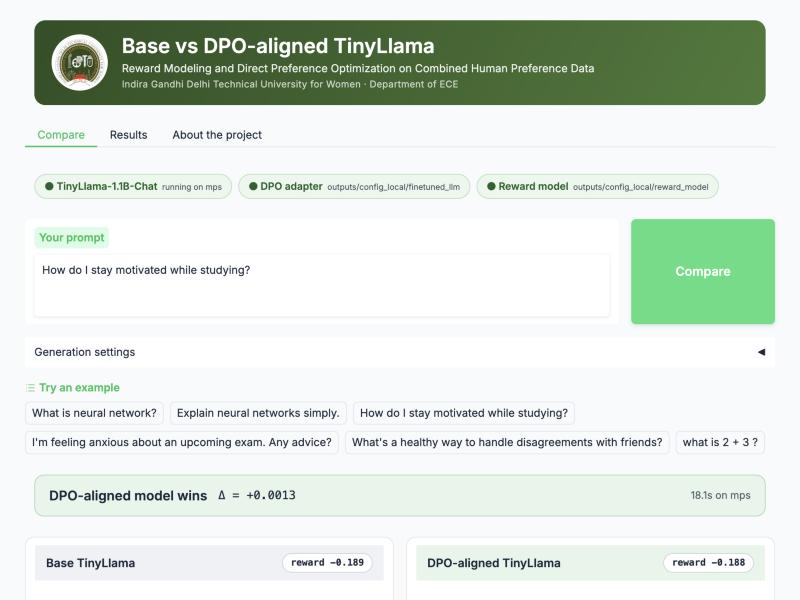
\includegraphics[width=0.92\textwidth]{figures/ui_compare_top.jpg}
\caption[Web application: Compare tab (input)]{Web application, Compare tab: model status, prompt box, example prompts and the result banner.}
\label{fig:ui-top}
\end{figure}

\begin{figure}[H]
\centering
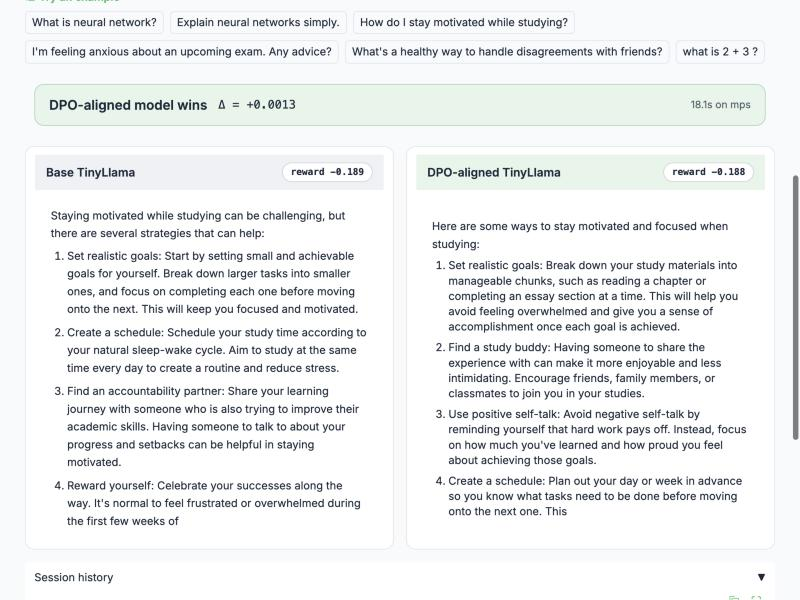
\includegraphics[width=0.92\textwidth]{figures/ui_compare_answers.jpg}
\caption[Web application: Compare tab (answers)]{Web application, Compare tab: base and DPO answers side by side with their reward scores.}
\label{fig:ui-answers}
\end{figure}

\begin{figure}[H]
\centering
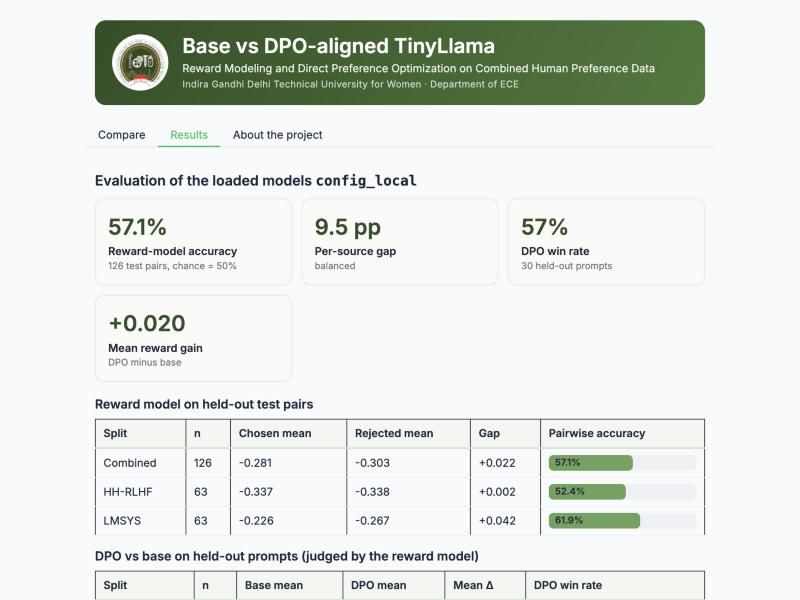
\includegraphics[width=0.92\textwidth]{figures/ui_results.jpg}
\caption[Web application: Results tab]{Web application, Results tab for the local configuration: summary tiles and per-source reward-model accuracy.}
\label{fig:ui-results}
\end{figure}

\begin{figure}[H]
\centering
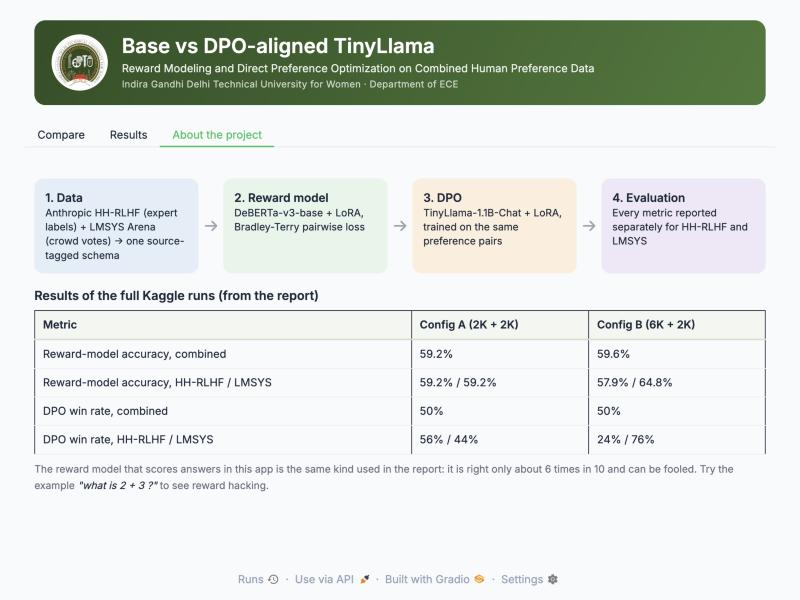
\includegraphics[width=0.92\textwidth]{figures/ui_about.jpg}
\caption[Web application: About tab]{Web application, About tab: pipeline overview and the results of the two Kaggle configurations.}
\label{fig:ui-about}
\end{figure}

\section{Engineering Challenges and Fixes}
\label{sec:impl-fixes}

Getting current versions of Transformers, TRL and PEFT to work on a T4, and later on an M1 laptop, threw up a series of problems, and several of them gave no error at all. Table~\ref{tab:fixes} lists them, and the most important ones are explained after the table.

{\footnotesize
\begin{longtable}{@{}L{0.5cm}L{4.0cm}L{4.3cm}L{5.0cm}@{}}
\caption[Implementation problems and fixes]{Problems encountered during implementation and their fixes.}\label{tab:fixes}\\
\toprule
\textbf{\#} & \textbf{Symptom} & \textbf{Root cause} & \textbf{Fix}\\
\midrule\endfirsthead
\toprule
\textbf{\#} & \textbf{Symptom} & \textbf{Root cause} & \textbf{Fix}\\
\midrule\endhead
\bottomrule\endfoot
1 & Reward scores are NaN; accuracy meaningless & DeBERTa-v3 disentangled attention overflows in FP16/BF16 & Load the RM in FP32 (fits easily at 184M parameters); NaN guards in scoring\\
2 & Crash in the FP16 gradient scaler: \texttt{NotImplementedError} \ldots\ \emph{not implemented for BFloat16} & TinyLlama's default BF16 layers + FP16 GradScaler; T4 lacks BF16 & FP16 compute for the 4-bit layers, FP16 for the remaining layers, mixed precision switched off in the trainers\\
3 & Reloaded RM gives different, unreliable scores from those seen in training & PEFT saved LoRA + classifier but \emph{not} the randomly initialised pooler; a fresh load re-randomises it & Add the pooler to \texttt{modules\_to\_save} so it is trained, saved and restored\\
4 & Old RM checkpoint fails to load after switching backbone & An adapter from the TinyLlama prototype was still in the working folder & First cell reads each \texttt{adapter\_config.json} and deletes checkpoints for the wrong backbone\\
5 & Device-mismatch errors on 2-GPU machine & Automatic placement put the model on \texttt{cuda:1} while inputs went to \texttt{cuda:0} & Send inputs to the device that holds the model's first parameter\\
6 & Validation and test sets overlapped & Same tail rows carved twice & Single-pass stratified split; disjoint slices\\
7 & Most LMSYS multi-turn rows disappeared & Over-length rows rejected rather than truncated & Truncate fields to 1,500 chars\\
8 & Cross-model context contamination & Earlier turns of A and B came from different models & Keep only the final user turn and final responses\\
9 & Attribute errors iterating LMSYS rows & Column names with trailing spaces; NaN values & Strip column names, check the schema, parse with \texttt{safe\_parse}\\
10 & Tokeniser crash on some LMSYS text & Unpaired UTF-16 surrogates & \texttt{clean\_text} removes them\\
11 & PEFT import error mentioning torchao & Kaggle ships torchao 0.10; PEFT needs $\ge$0.16 & Force-reinstall torchao and purge it from \texttt{sys.modules}\\
12 & TRL import crash & wandb/protobuf version mismatch & Upgrade wandb and disable it with environment variables\\
13 & Trained models lost between sessions & \texttt{/kaggle/working} is wiped & Save a notebook version and auto-detect adapters among the input datasets\\
14 & Gradient-checkpointing error with LoRA RM & Inputs did not require grad for non-quantised PEFT model & Call \texttt{enable\_input\_}\allowbreak\texttt{require\_grads()} on the model\\
15 & DPO over-fitting, later epochs degrade (config B) & High LR, too many epochs & LR $5\!\times\!10^{-5}\!\to\!10^{-5}$, $\beta$ 0.1$\to$0.15, best-checkpoint reload\\
16 & DPO stopped at step 3 on the 8\,GB M1 with an MPS ``Insufficient Memory'' error & FP16 TinyLlama plus two sequences per step exceeded unified memory & One pair per step with 8-step accumulation, 256-token DPO inputs, and the MPS memory cap lifted with an environment variable (Appendix~\ref{app:repro})\\
17 & LMSYS file not available outside Kaggle & Competition data needs a Kaggle login & Download the identical public copy (\texttt{lmarena-ai/}\allowbreak\texttt{arena-human-preference-55k}) from the HuggingFace Hub\\
\end{longtable}
}

\paragraph{The pooler problem (fix 3).} This was the hardest bug to find. In DeBERTa the classification head is a pooler followed by a classifier. Neither is part of the downloaded checkpoint (the loading report marks both \texttt{MISSING}), so both start with random values. With \texttt{TaskType.SEQ\_CLS}, PEFT trains and saves the classifier on its own, but the pooler, with 590,592 parameters, stayed frozen at its random start and was never saved. When a later cell loaded the reward model again, it received a \emph{new} random pooler, and the trained adapters and classifier were now attached to a layer they had never seen. As a result, scores at evaluation time did not match scores during training. Adding \texttt{modules\_to\_save=[\textquotedbl{}pooler\textquotedbl{}]} makes the pooler trainable, stores it with the adapter, and \texttt{PeftModel.from\_pretrained} puts it back exactly.

\paragraph{Number formats (fixes 1, 2 and 16).} Our two models need opposite settings. DeBERTa-v3 has to run in FP32 because its attention overflows in 16-bit. TinyLlama's 4-bit layers have to compute in FP16, because the T4 cannot do BF16 and mixing BF16 weights with an FP16 gradient scaler crashes. Turning off the trainers' mixed-precision options removes the gradient scaler completely, and memory is already saved by the 4-bit weights and LoRA. On the 8\,GB M1 laptop the policy cannot be quantised (bitsandbytes needs CUDA), so it runs in plain FP16, and DPO had to be cut to one pair per step with 256-token inputs to fit.

\section{Summary}
In this chapter we walked through the ten modules: the environment and saving logic, the two dataset parsers, the shared filter and per-source split, the DeBERTa-v3 reward model, 4-bit DPO training of TinyLlama, and the generation, evaluation and live-demo code. We then showed how this code became a reusable package and web application, listed the settings of every configuration, and recorded the problems we fixed. Some of them, such as the unsaved pooler, would have silently ruined the evaluation if they had not been caught. Chapter~\ref{ch:results} presents the results.
